\section{Pruebas}
Para comprobar el funcionamiento del programa se ingreso la siguiente señal (como archivo wav):
\begin{figure}[H]
	\centering
	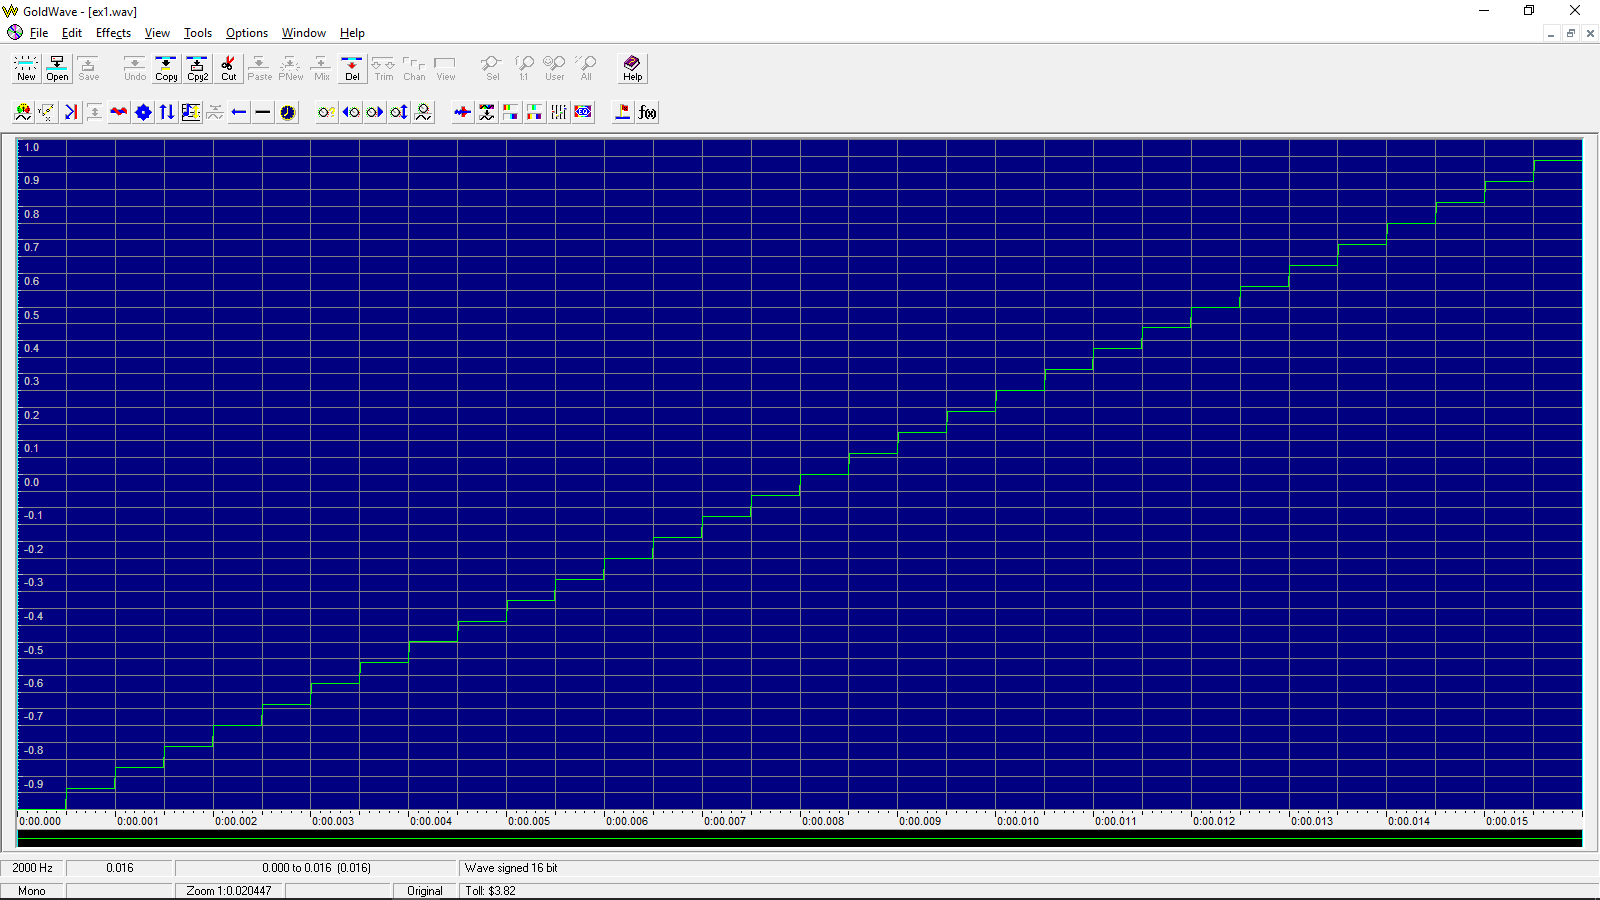
\includegraphics[scale=.3]{img/prueba1.png}
	\caption{Entrada 1}
	\label{fig:prueba1}		
\end{figure}
Salida obtenida:
\begin{figure}[H]
	\centering
	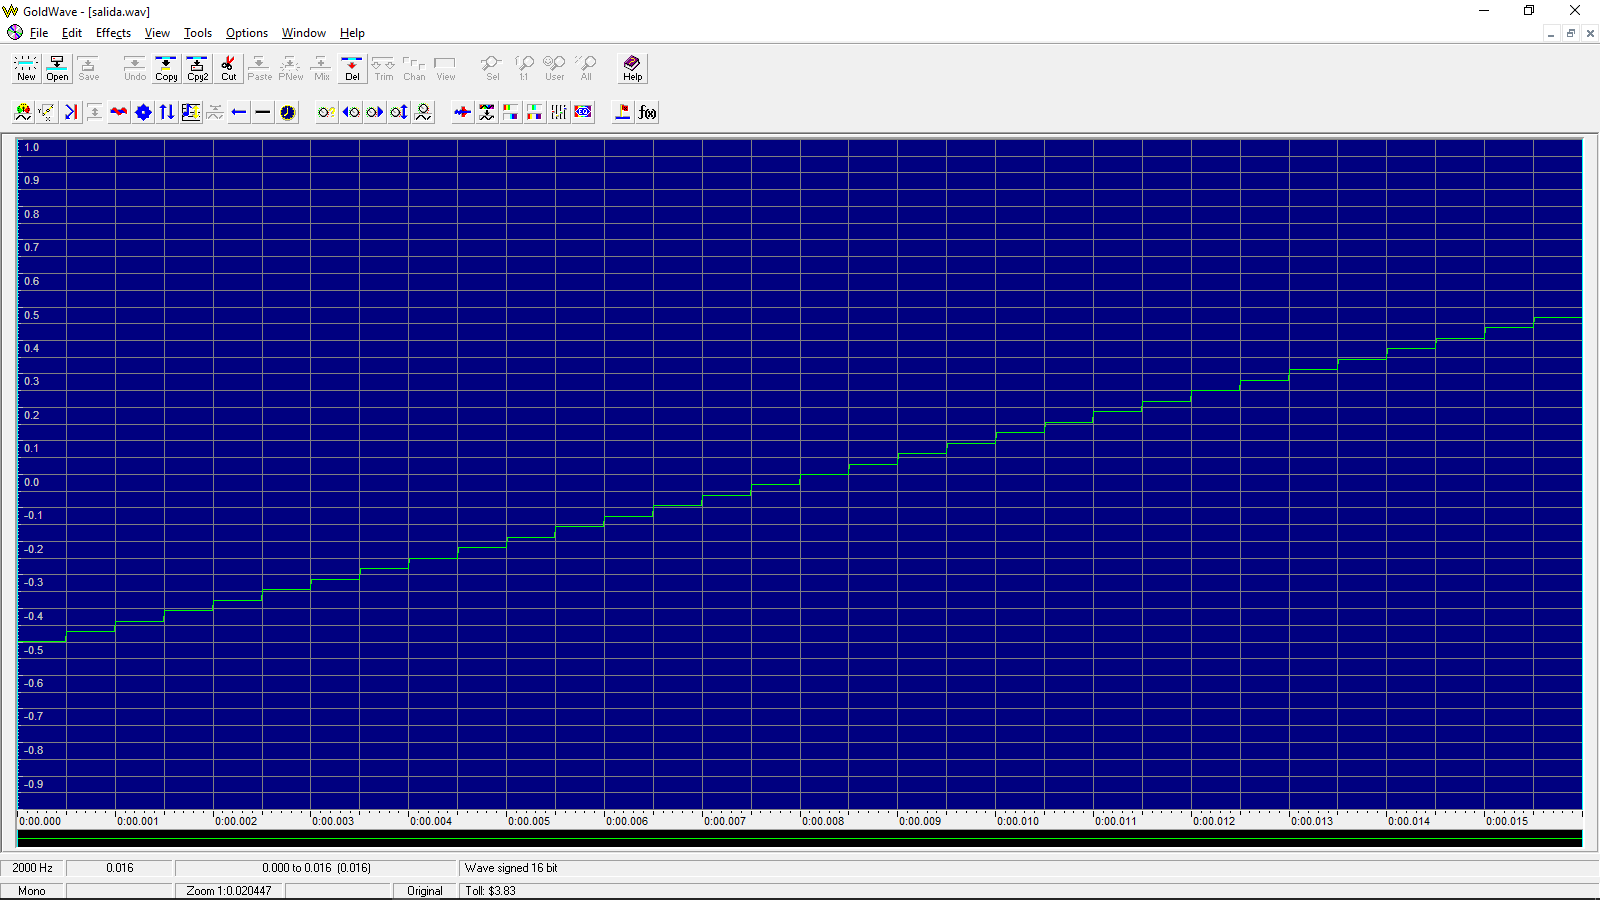
\includegraphics[scale=.3]{img/salida1.png}
	\caption{Salida 1}
	\label{fig:salida1}		
\end{figure}
Posteriormente, se probó el programa con la siguiente señal de entrada:
\begin{figure}[H]
	\centering
	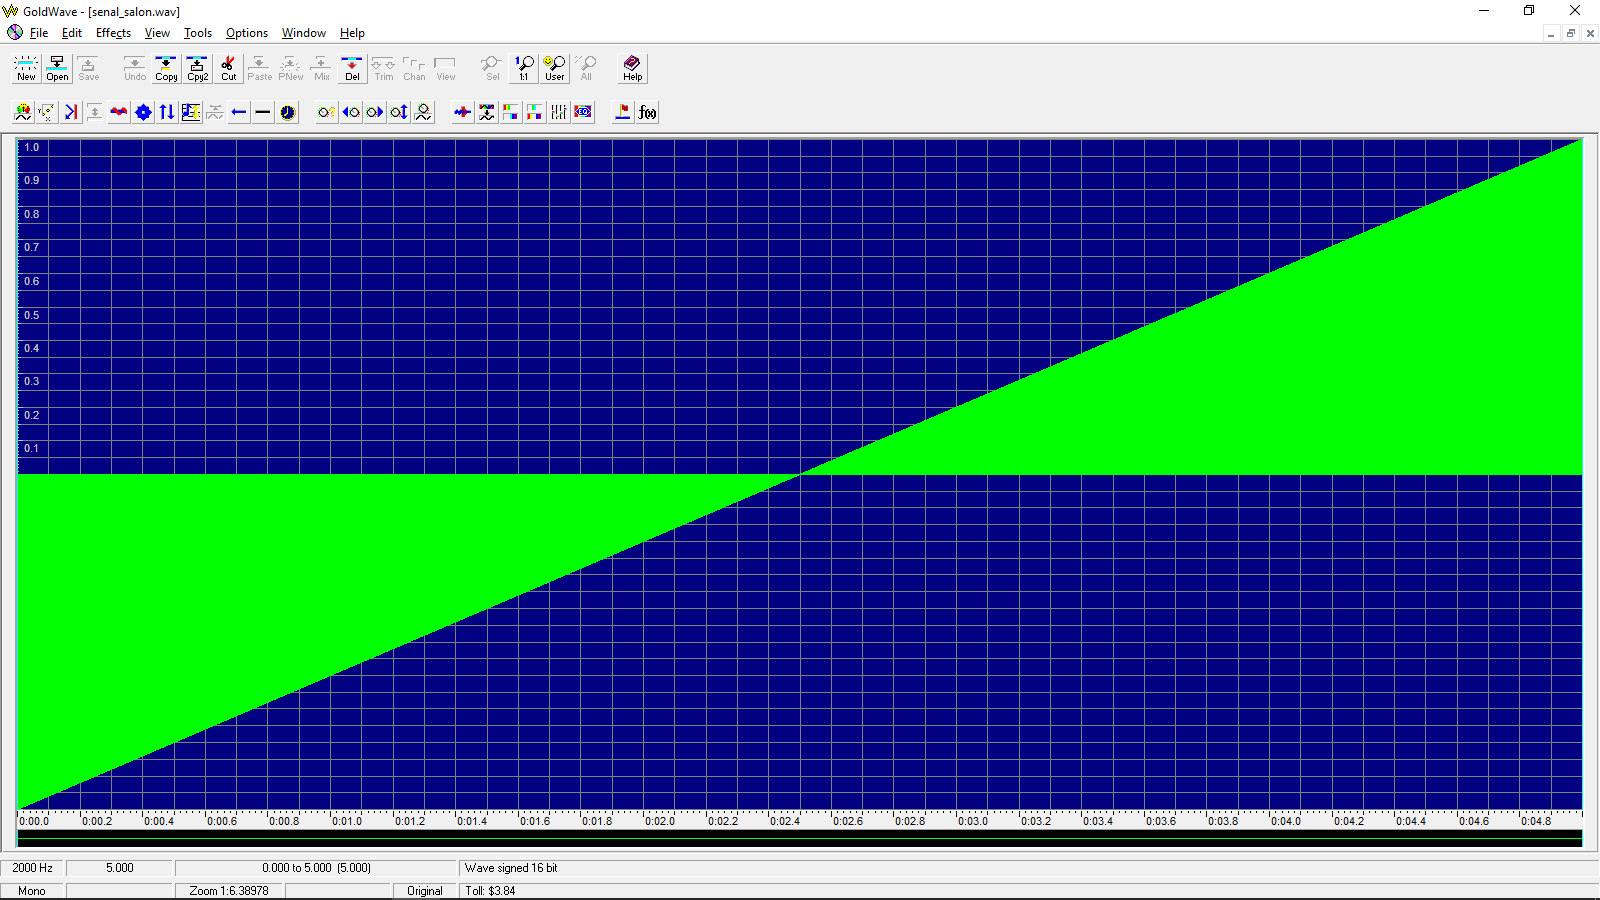
\includegraphics[scale=.3]{img/prueba2.png}
	\caption{Entrada 2}
	\label{fig:prueba2}		
\end{figure}
Salida obtenida:
\begin{figure}[H]
	\centering
	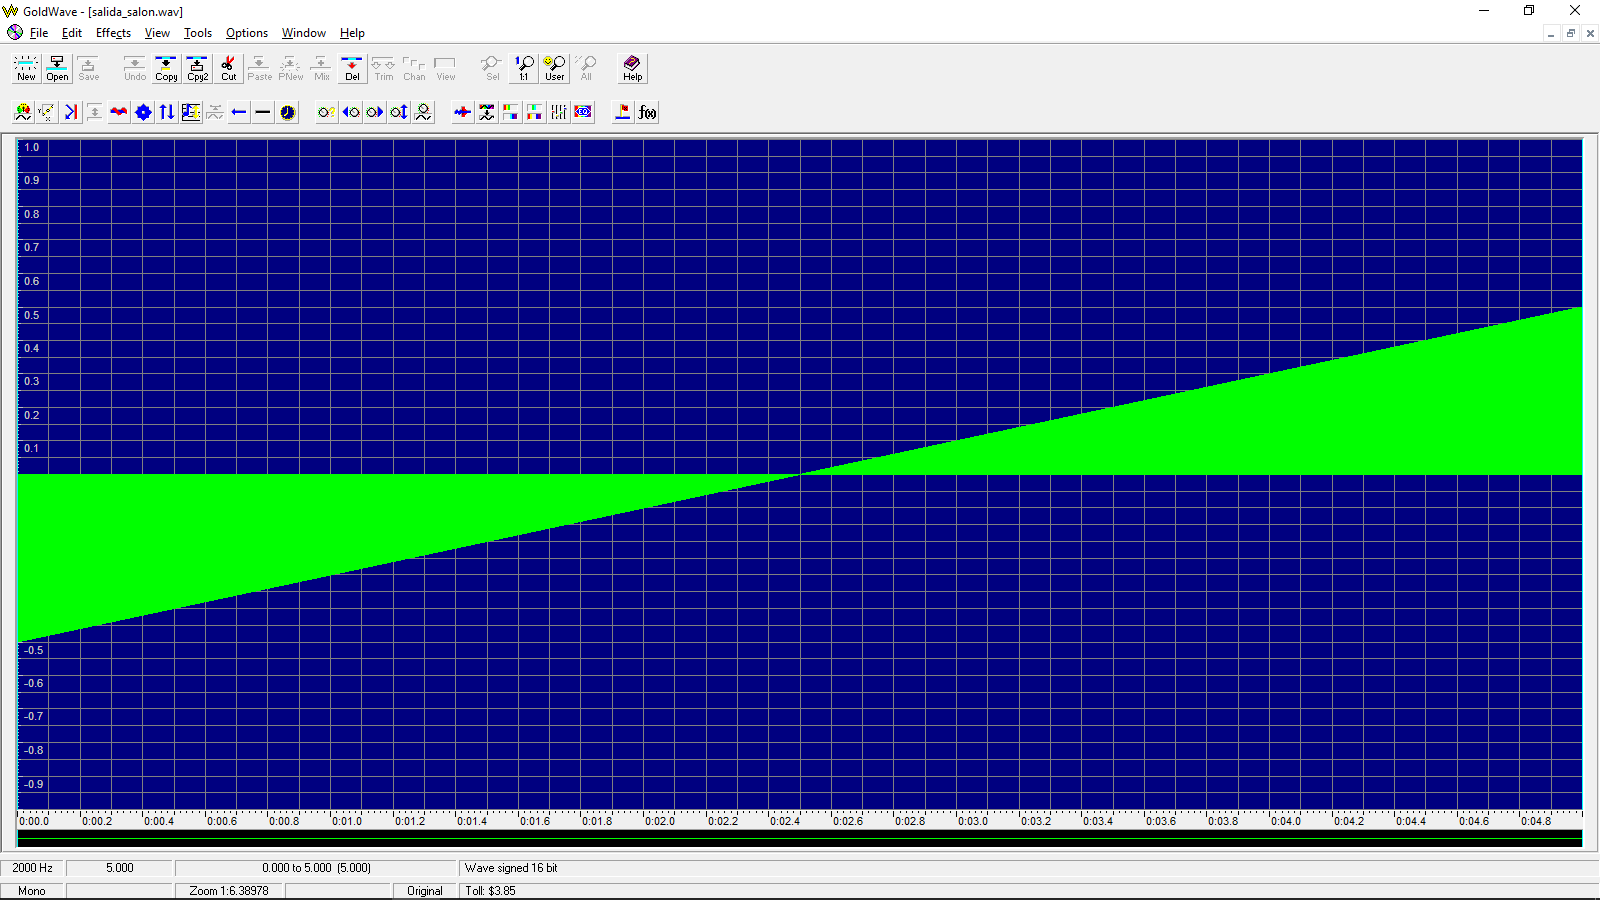
\includegraphics[scale=.3]{img/salida2.png}
	\caption{Salida 2}
	\label{fig:salida2}		
\end{figure}